\documentclass[a4paper]{IEEEtran}

% Ein paar hilfreiche Pakete
\usepackage[utf8]{inputenc}
\usepackage[nenglish]{babel}
\usepackage{graphicx}
\usepackage{amsmath}
\usepackage{amssymb}
\usepackage{mathtools}
\usepackage{subcaption}
\usepackage{hyperref}

\mathtoolsset{showonlyrefs}

\markboth{Proseminar WS 18/19: Anthropomatik: Von der Theorie zur Anwendung}{Proseminar SS 16: Anthropomatik: Von der Theorie zur Anwendung}

% Hier den Titel des eigenen Proseminars eitnragen
\title{Discovery of Processes / Process Minining}

% Hier deinen eigenen Namen
\author{Maximilian Franz}


\begin{document}
\maketitle

% Zusammenfassung
\begin{abstract}
TODO
\end{abstract}

\section{Notes}
Preliminary Notes throughout research. \newline
\textbf{Possible Outline}
\begin{enumerate}
\item Introduction - Importance of ProcessMining
    \item Introduce the Task of Process Mining and Notation
    \item $\alpha$-algorithm
    \item Other algorithms
    \item comparison 
    \item implementation 
\end{enumerate}

% Erster Abschnitt
\section{Introduction}
\begin{itemize}
    \item The importance and usage of process mining 
    \item The difficulties and problems of process mining
\end{itemize}
Errors of \textbf{Process Modelling} include
\begin{itemize}
    \item The model describes an idealized version of reality.
    \item Human behaviour cannot be captured in simple stated forms
    \item The model is at the wrong abstraction level. 
\end{itemize}
Thus process mining can facilitate the construction of better models in less time \cite{process_mining}. \newline

\section{Notation and Terminology}
Introduce important notations in formula and terminology around processes

\begin{itemize}

    \item \textbf{Process} -  \textbf{Case}
    \item \textbf{Petri Nets} and WF-Nets 
    \item \textbf{Logs} and Data Notation
    \item \textbf{Process Discovery Problem Statement}
\end{itemize}
\textbf{Logs:} Events are $e \in \mathcal{E}$
\begin{figure}[!h]
    \centering
    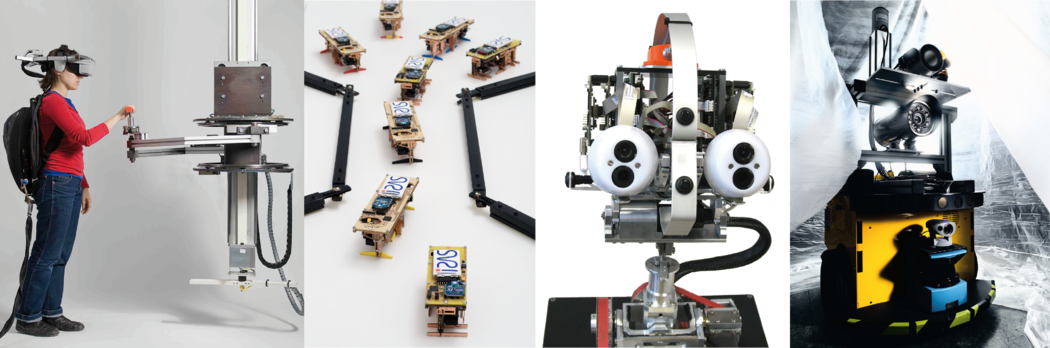
\includegraphics[width=0.48\textwidth]{Bild.png}
    \caption{Hier kommen weitere Erklärungen zum Bild.}
    \label{fig:bild}
\end{figure}


\bibliographystyle{ieeetr}
\bibliography{references}
\end{document}
